\subsection{Performance of the BELLA model}

We assessed the performance of our model through analyses of a diverse set of simulated datasets (\ref{subsec:sim-study}), and showed that BELLA reliably achieved accurate results in both epidemiological and macroevolutionary contexts.
\rv{
    We tested different fully connected neural network architectures by varying the number of hidden layers and nodes, the activation functions, and the priors on the weights (Table \ref{tab:models}).
    The resulting BELLA models included between 20 and 705 weights, depending on the number of predictors and model architecture.
    Hereafter, we report results from a network with two hidden layers of 16 and 8 nodes, ReLU activation functions, and standard normal priors on the weights (\texttt{BELLA-3} in Tab.~\ref{tab:models}).
    This architecture provided one of the best compromises between coverage and accuracy across the datasets considered. Additional results for all evaluated models are provided in the \textit{Supplementary Information}.
}

The simulation scenarios included a varied suite of predictor--parameter relationships, encompassing constant, linear, and nonlinear dependencies applied to the reproduction number and migration rates (epidemiology; Fig.~\ref{fig:scenarios}a--d), as well as to speciation and extinction rates (macroevolution; Fig.~\ref{fig:scenarios}e--h). 
We evaluated the relative performance of the BELLA models by analyzing all simulated datasets under state-of-the-art alternatives, including ``predictor-agnostic'' models, in which rate variation is modeled using parameters that vary independently across time or lineages (for instance, piecewise-constant rates through time)~\cite{stadler2013birth, Vaughan2025BDMM}, and generalized linear models (GLMs) that modulate rate variation through log-linear correlations with the predictors~\citep{lemey2014unifying,muller2019inferring,valenzuela2021comprehensive}.
\rv{
    Model performance was assessed using mean absolute percentage error (MAPE), coverage, and the coefficient of variation (Tab.~\ref{tab:mape}–\ref{tab:cv}, Fig.~\ref{fig:metrics:mape}–\ref{fig:metrics:cv}). MAPE quantifies average relative prediction error, providing a scale-independent measure of accuracy across simulations; coverage measures the proportion of true values falling within the model’s predictive or credible intervals, serving as a proxy for uncertainty calibration; and the coefficient of variation captures relative dispersion of estimates, acting as a proxy for precision and stability of inferred rates across replicates.
}

% Constant and linear scenarios
\rv{
    We first evaluated the performance of the BELLA model under simulation scenarios in which the predictor–parameter relationship was either constant (Fig.~\ref{fig:scenarios}a,e) or linear (Fig.~\ref{fig:scenarios}b,f). Time and a random time series were included as predictors, but neither introduced detectable bias in the inferred parameters.
    These settings are well aligned with the assumptions of the GLM, whereas the greater flexibility of BELLA---in terms of both a higher number of parameters and a less constrained functional form---could, in principle, lead to overfitting. Despite this, both the GLM and BELLA accurately and precisely recovered the true rates (Figs.~\ref{fig:epi-skyline:ribbons}a--b, \ref{fig:fbd-no-traits:ribbons}a--b).
    The mean absolute percentage error (MAPE) was comparable between the two approaches for both reproduction numbers and speciation and extinction rates. Coverage remained close to or above 0.95 across methods, indicating that true parameter values were consistently contained within posterior credible intervals across all time bins. However, GLMs generally exhibited a slightly lower coefficient of variation, reflecting higher precision in parameter estimates.
    In contrast, the predictor-agnostic model—which estimates independent phylodynamic parameters in each of the ten time bins—showed higher error and reduced coverage, with particularly poor performance in early time bins (Figs.~\ref{fig:epi-skyline:metrics}a--b, \ref{fig:fbd-no-traits:metrics}a--b). This behavior likely reflects overfitting arising from the absence of regularization or explicit model selection constraints.
}

% Interacting predictors
\rv{
We also evaluated BELLA under a macroevolutionary scenario in which both speciation and extinction rates varied through time and across lineages as a function of a binary trait evolving along the phylogeny (Fig.~\ref{fig:scenarios}h), as well as a time series that induced a transient spike in extinction rates. In this setting, predictors interact, making inference substantially more challenging.
The GLM, constrained by its functional form, was unable to disentangle the combined effects of the trait and temporal predictors, resulting in poor estimates of speciation rates (Fig.~\ref{fig:fbd-2traits:benchmark}b). In contrast, BELLA recovered the true rate dynamics more accurately (Fig.~\ref{fig:fbd-2traits:summary}c), achieving comparable MAPE (0.23 vs. 0.27) but substantially improved coverage (0.96 vs. 0.72 for the GLM), indicating more reliable uncertainty quantification under interacting predictor effects.
}

\begin{figure}[htpb]
    \centering
    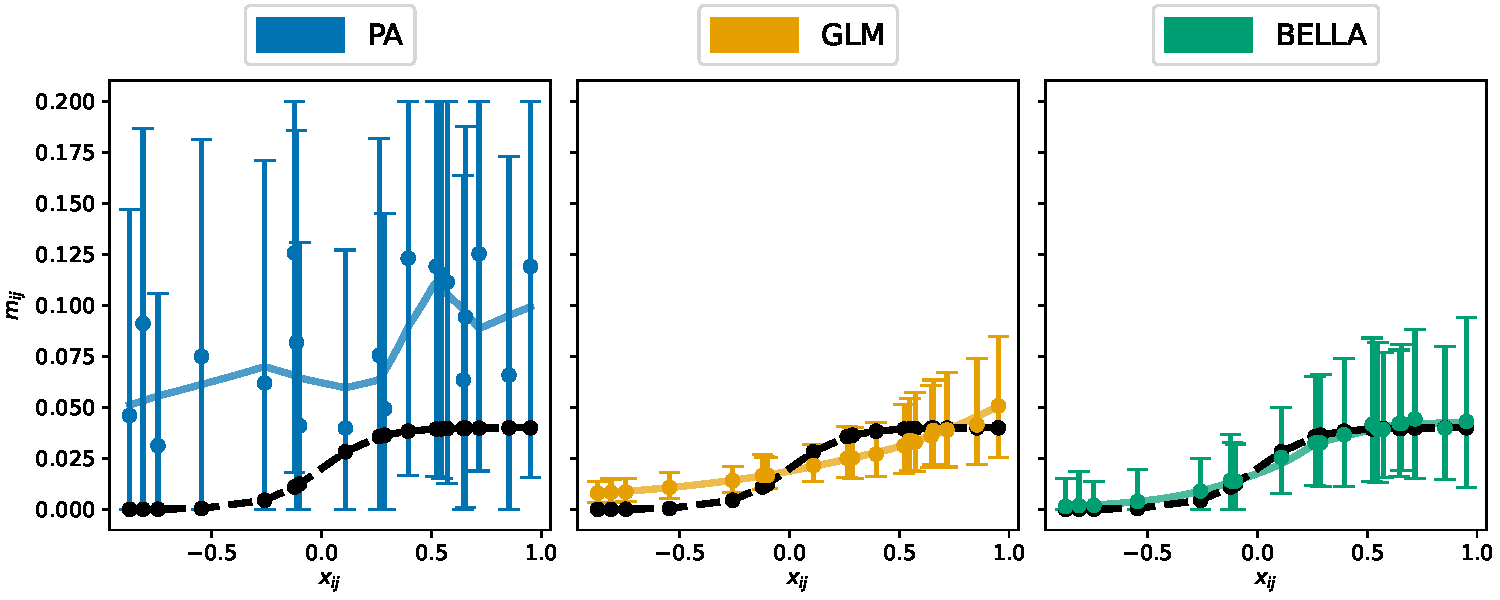
\includegraphics[width=1\textwidth]{figures/epi-multitype/summary.pdf}
    \caption{
    Results for a simulation scenario involving the prediction of 20 migration rates among all pairs of 5 populations (\texttt{Epi-4}) across 100 simulation replicates, evaluated across the inference frameworks considered.. Migration rates $m_{ij}$ were modeled based on a logistic function of an input predictor $x_{ij}$. In each panel, points and vertical intervals show the across-replicate median posterior estimate and interval bounds for each directed migration rate, plotted against its migration predictor; the colored smooth curve summarizes the fitted predictor-rate trend, and the black dashed curve with points shows the true simulated migration rates. \rv{The BELLA estimates are based on an architecture with two hidden layers of 16 and 8 nodes, ReLU activation functions, and standard normal priors on the weights (\texttt{BELLA-3} in Tab.~\ref{tab:models}).}
    }
    \label{fig:epi-multitype:summary}
\end{figure}

% Non-linear scenarios
Finally, we assessed the performance of BELLA in scenarios with nonlinear predictor-parameter relationships. These included epidemiological simulations with non-monotonic reproduction numbers over time (Fig.~\ref{fig:scenarios}c) and logistic patterns of migration rates (Fig.~\ref{fig:scenarios}d), as well as macroevolutionary simulations featuring declining speciation rates and spiking extinction rates (Fig.~\ref{fig:scenarios}g). 
\rv{
    In these complex settings, BELLA successfully captured the non-linear rate patterns (Figs.\ref{fig:epi-multitype:summary},~\ref{fig:epi-skyline:ribbons}c,~\ref{fig:fbd-no-traits:ribbons}c), achieving substantially better estimates compared to the other models. For example, migration rates estimated with BELLA (MAPE = 0.36) were substantially more accurate than those obtained under the predictor-agnostic model (MAPE = 2.25), while GLM estimates showed poorer uncertainty calibration, with lower coverage (0.59) compared to BELLA (0.97).
    Similarly, the MAPE of estimated speciation and extinction rates improved three-fold under BELLA compared with the alternative approaches, although coverage was lower than under the predictor-agnostic model (0.855 vs 0.97), indicating a slight underestimation of uncertainty around the single-time-bin peak (Fig.~\ref{fig:fbd-no-traits:ribbons}c).
}

\rv{
    BELLA estimates across simulations were generally consistent across model architectures varying in the number of hidden layers, number of nodes, activation functions, and priors on the weights (Tab.~\ref{tab:models}). MAPE and coverage levels showed relatively little variation among model configurations, suggesting that parameter estimates were robust (Figs.~\ref{fig:metrics:mape},~\ref{fig:metrics:coverage}) and providing little evidence of overfitting, even when using relatively large neural networks (Figs.~\ref{fig:epi-skyline:sensitivity:epi-skyline_1}--\ref{fig:epi-multitype:sensitivity},~\ref{fig:fbd-no-traits:sensitivity:fbd-no-traits_1}--\ref{fig:fbd-no-traits:sensitivity:fbd-no-traits_3}). However, the use of a very small network (\texttt{BELLA-2}, with two hidden layers of 3 and 2 nodes, respectively) appeared to limit the model's ability to fit complex scenarios involving multiple interacting predictors (Fig.~\ref{fig:fbd-2traits:sensitivity}a), although it still performed well in simulations with simpler mapping functions. Similarly, the use of sigmoid activation functions in the hidden layers (\texttt{BELLA-8}) led, in some cases, to a flattening of the inferred relationships (Figs.~\ref{fig:epi-multitype:sensitivity},~\ref{fig:fbd-no-traits:sensitivity:fbd-no-traits_3}b,~\ref{fig:fbd-2traits:sensitivity}a).
}
    